\begingroup
\graphicspath{{../prob_1/Figures/}}

% =====================================================
% Problem 1 : Conditional VAE for MNIST Data Generation
% =====================================================

\subsection{Conditional Variational Autoencoder (VAE)}

In this experiment, a Conditional Variational Autoencoder (CVAE) was implemented to generate synthetic MNIST handwritten digit images using only a limited real dataset of 350 samples per digit.

The main objective was to investigate whether synthetic data generated by a VAE can improve the performance of a LeNet-5 classifier trained on a small dataset.

% =====================================================
\subsubsection{Pipeline Overview}

The implemented pipeline is summarized as follows:

\begin{enumerate}
    \item Load and preprocess MNIST dataset.
    
    \item Reduce the training dataset to only 350 real samples per digit.
    
    \item Apply data augmentation using:
    \begin{itemize}
        \item Rotation
        \item Translation
        \item Scaling
        \item Gaussian noise
    \end{itemize}
    
    \item Train a Conditional VAE using the augmented dataset.
    
    \item Repeat VAE training for 5 independent runs using different random weight initialization.
    
    \item Generate 1000 synthetic images per digit from each VAE run.
    
    \item Train a LeNet-5 classifier using only the 350 real samples.
    
    \item Classify generated samples and compute:
    
    \[
    \text{confidence} = \max(\text{softmax output})
    \]
    
    \item Create three synthetic datasets:
    
    \begin{itemize}
        \item Set A: all generated samples
        \item Set B: confidence $\geq 0.9$
        \item Set C: $0.6 \leq$ confidence $< 0.9$
    \end{itemize}
    
    \item Retrain LeNet-5 using:
    \begin{itemize}
        \item 350 real samples only
        \item 350 real + Set A
        \item 350 real + Set B
        \item 350 real + Set C
    \end{itemize}
    
    \item Compare against:
    \begin{itemize}
        \item 350-real baseline
        \item 1000-real baseline
    \end{itemize}
    
\end{enumerate}

% =====================================================
% =====================================================
\subsubsection{Pipeline Flowchart}

\definecolor{softblue}{RGB}{173,216,230}
\definecolor{softgreen}{RGB}{190,230,200}
\definecolor{softpurple}{RGB}{220,210,255}
\definecolor{softorange}{RGB}{255,220,180}
\definecolor{softred}{RGB}{255,200,200}

\begin{figure}[H]
\centering

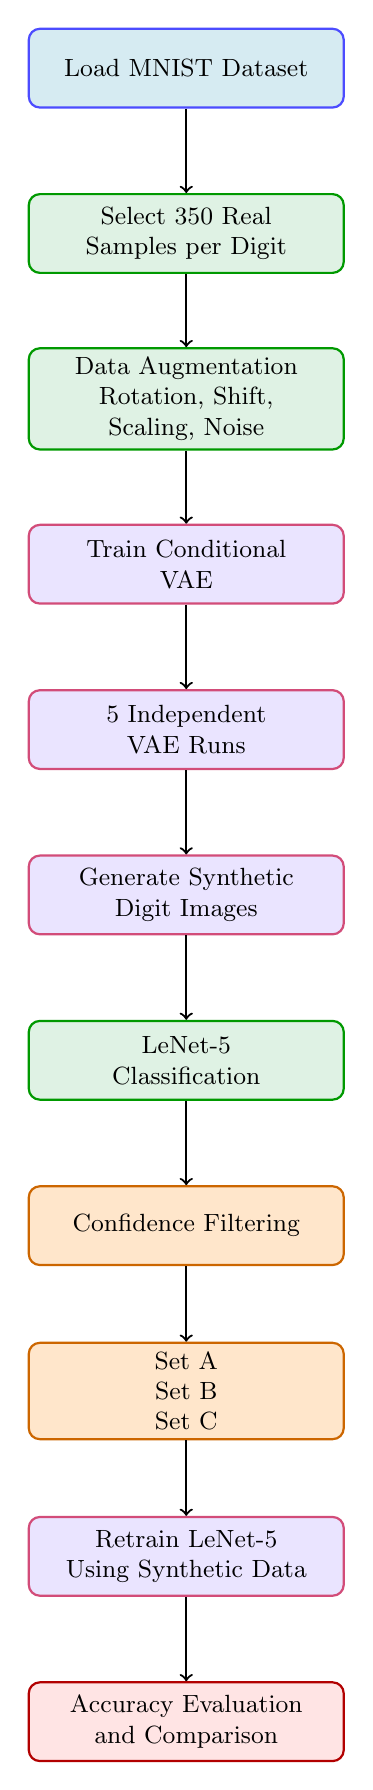
\begin{tikzpicture}[
node distance=2.1cm,
every node/.style={
align=center,
minimum width=4cm,
minimum height=1cm,
font=\small
},
arrow/.style={->, thick}
]

% =====================================================
% Styles
% =====================================================

\tikzstyle{input} =
[rectangle, rounded corners,
fill=softblue!50,
draw=blue!70,
thick]

\tikzstyle{process} =
[rectangle, rounded corners,
fill=softgreen!50,
draw=green!60!black,
thick]

\tikzstyle{model} =
[rectangle, rounded corners,
fill=softpurple!60,
draw=purple!70,
thick]

\tikzstyle{filter} =
[rectangle, rounded corners,
fill=softorange!70,
draw=orange!80!black,
thick]

\tikzstyle{output} =
[rectangle, rounded corners,
fill=softred!50,
draw=red!70!black,
thick]

% =====================================================
% Nodes
% =====================================================

\node (mnist) [input]
{Load MNIST Dataset};

\node (reduce) [process, below of=mnist]
{Select 350 Real\\Samples per Digit};

\node (augment) [process, below of=reduce]
{Data Augmentation\\Rotation, Shift,\\Scaling, Noise};

\node (trainvae) [model, below of=augment]
{Train Conditional\\VAE};

\node (runs) [model, below of=trainvae]
{5 Independent\\VAE Runs};

\node (generate) [model, below of=runs]
{Generate Synthetic\\Digit Images};

\node (classifier) [process, below of=generate]
{LeNet-5\\Classification};

\node (confidence) [filter, below of=classifier]
{Confidence Filtering};

\node (sets) [filter, below of=confidence]
{Set A\\Set B\\Set C};

\node (retrain) [model, below of=sets]
{Retrain LeNet-5\\Using Synthetic Data};

\node (evaluate) [output, below of=retrain]
{Accuracy Evaluation\\and Comparison};

% =====================================================
% Arrows
% =====================================================

\draw [arrow] (mnist) -- (reduce);

\draw [arrow] (reduce) -- (augment);

\draw [arrow] (augment) -- (trainvae);

\draw [arrow] (trainvae) -- (runs);

\draw [arrow] (runs) -- (generate);

\draw [arrow] (generate) -- (classifier);

\draw [arrow] (classifier) -- (confidence);

\draw [arrow] (confidence) -- (sets);

\draw [arrow] (sets) -- (retrain);

\draw [arrow] (retrain) -- (evaluate);

\end{tikzpicture}

\caption{Colored pipeline of the Conditional VAE synthetic data generation framework.}

\label{fig:vae_pipeline}

\end{figure}

% =====================================================
\subsubsection{Original MNIST Samples}

Figure~\ref{fig:mnist_samples} shows examples from the original MNIST dataset.

\begin{figure}[H]
\centering
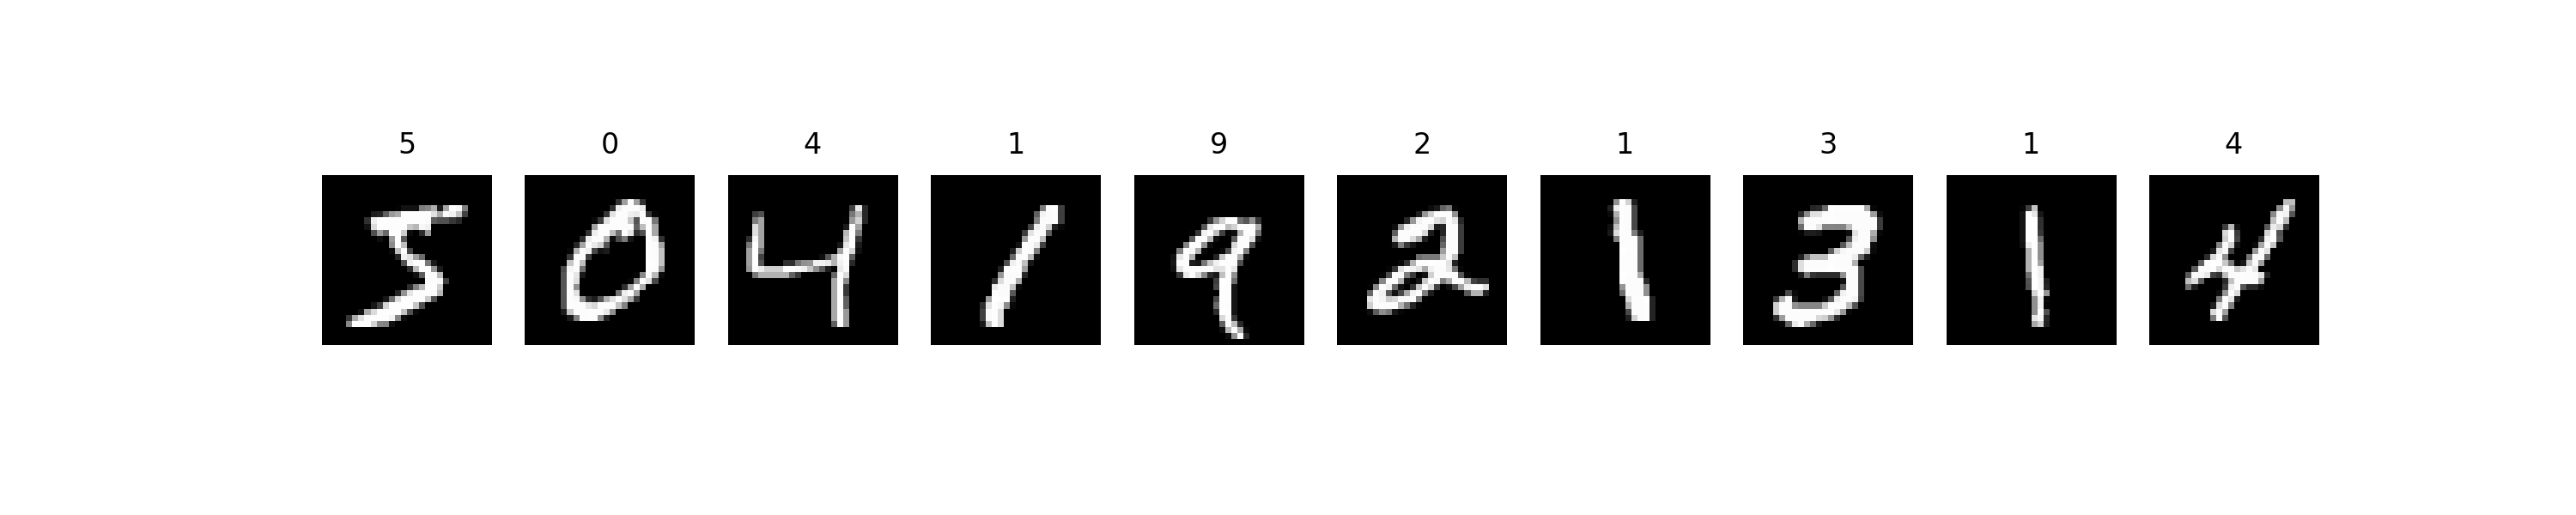
\includegraphics[width=0.95\linewidth]{MNIST_samples.png}
\caption{Original MNIST samples.}
\label{fig:mnist_samples}
\end{figure}

% =====================================================
\subsubsection{Data Augmentation}

To compensate for the limited dataset size, multiple augmentation techniques were applied.

These augmentations improve generalization and help the VAE learn digit variations.

Figure~\ref{fig:vae_aug} shows augmented examples.

\begin{figure}[H]
\centering
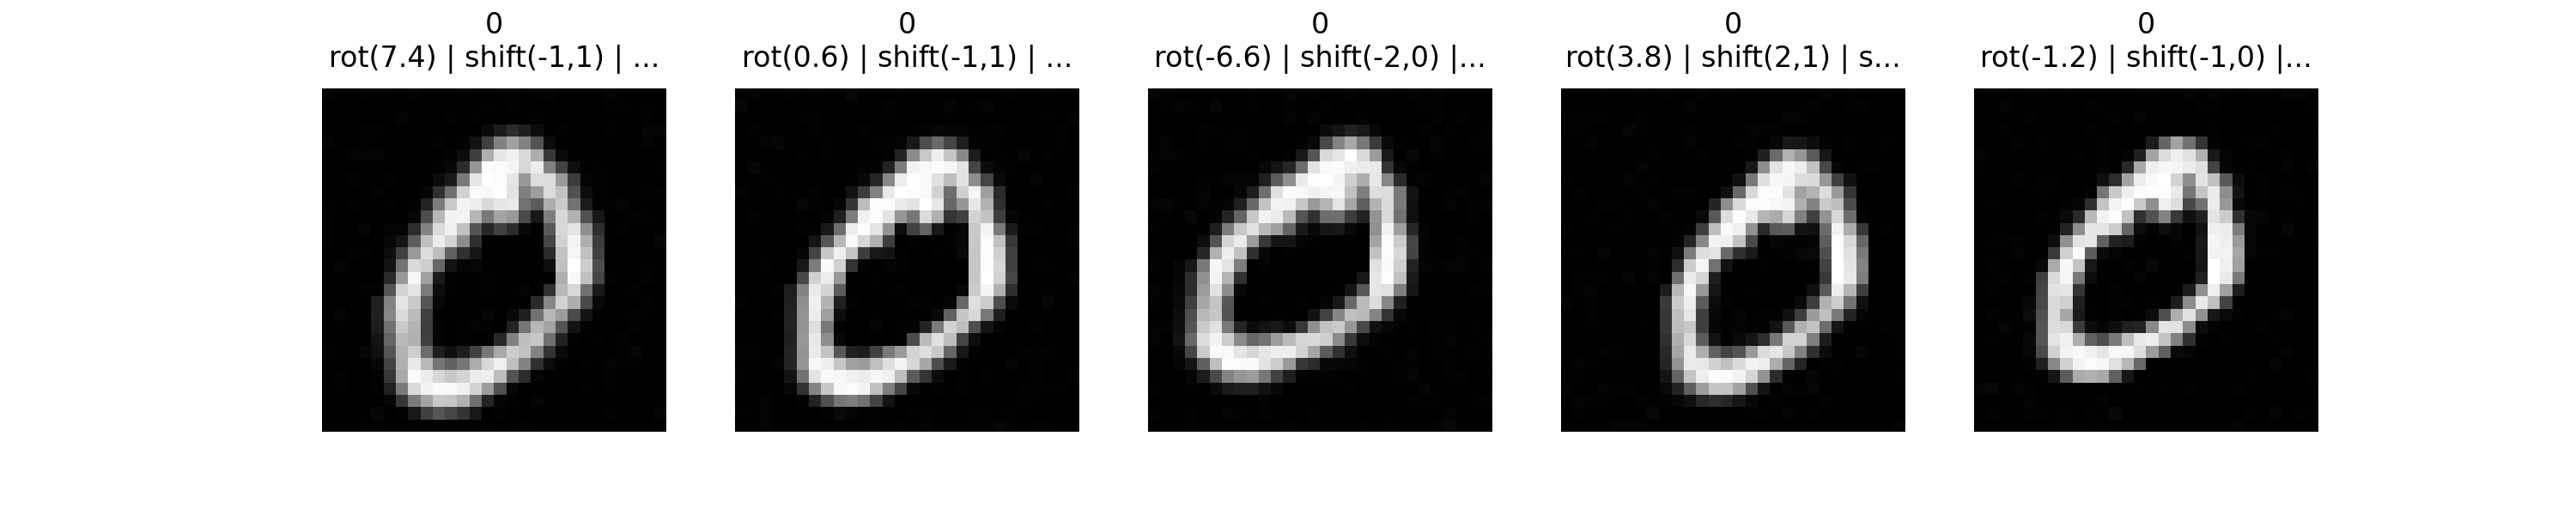
\includegraphics[width=\linewidth]{vae_aug_samples.png}
\caption{Examples of augmented MNIST samples using rotation, shifting, scaling, and noise injection.}
\label{fig:vae_aug}
\end{figure}

% =====================================================
\subsubsection{VAE Architecture}

The implemented Conditional VAE consists of:

\begin{itemize}
    \item Encoder:
    \begin{itemize}
        \item Convolutional layers
        \item Latent mean and variance estimation
    \end{itemize}
    
    \item Decoder:
    \begin{itemize}
        \item Dense projection
        \item Reshape layer
        \item Transposed convolution layers
        \item Sigmoid output layer
    \end{itemize}
\end{itemize}

The latent dimension was selected as:

\[
z \in \mathbb{R}^{8}
\]

The loss function combines:

\begin{itemize}
    \item Binary Cross Entropy reconstruction loss
    \item KL-divergence regularization
\end{itemize}

% =====================================================
\subsubsection{Generated Samples During Training}

Five independent VAE runs were trained using different random initialization.

Figures~\ref{fig:vae_run1} -- \ref{fig:vae_run5} show generated samples from different runs.

\begin{figure}[H]
\centering
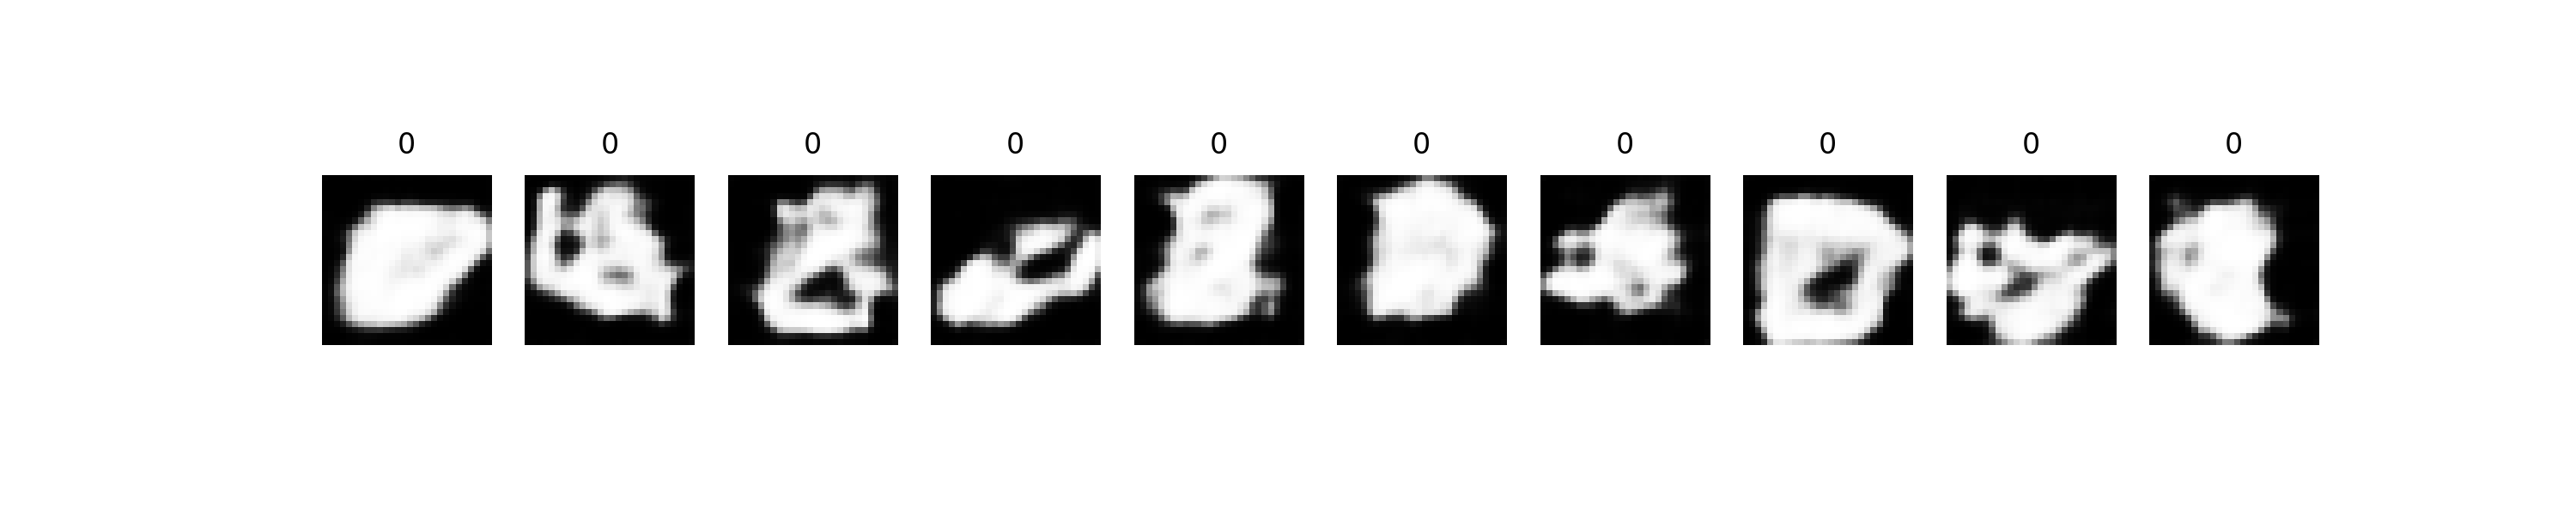
\includegraphics[width=\linewidth]{vae_run_1.png}
\caption{Generated samples from VAE Run 1.}
\label{fig:vae_run1}
\end{figure}

\begin{figure}[H]
\centering
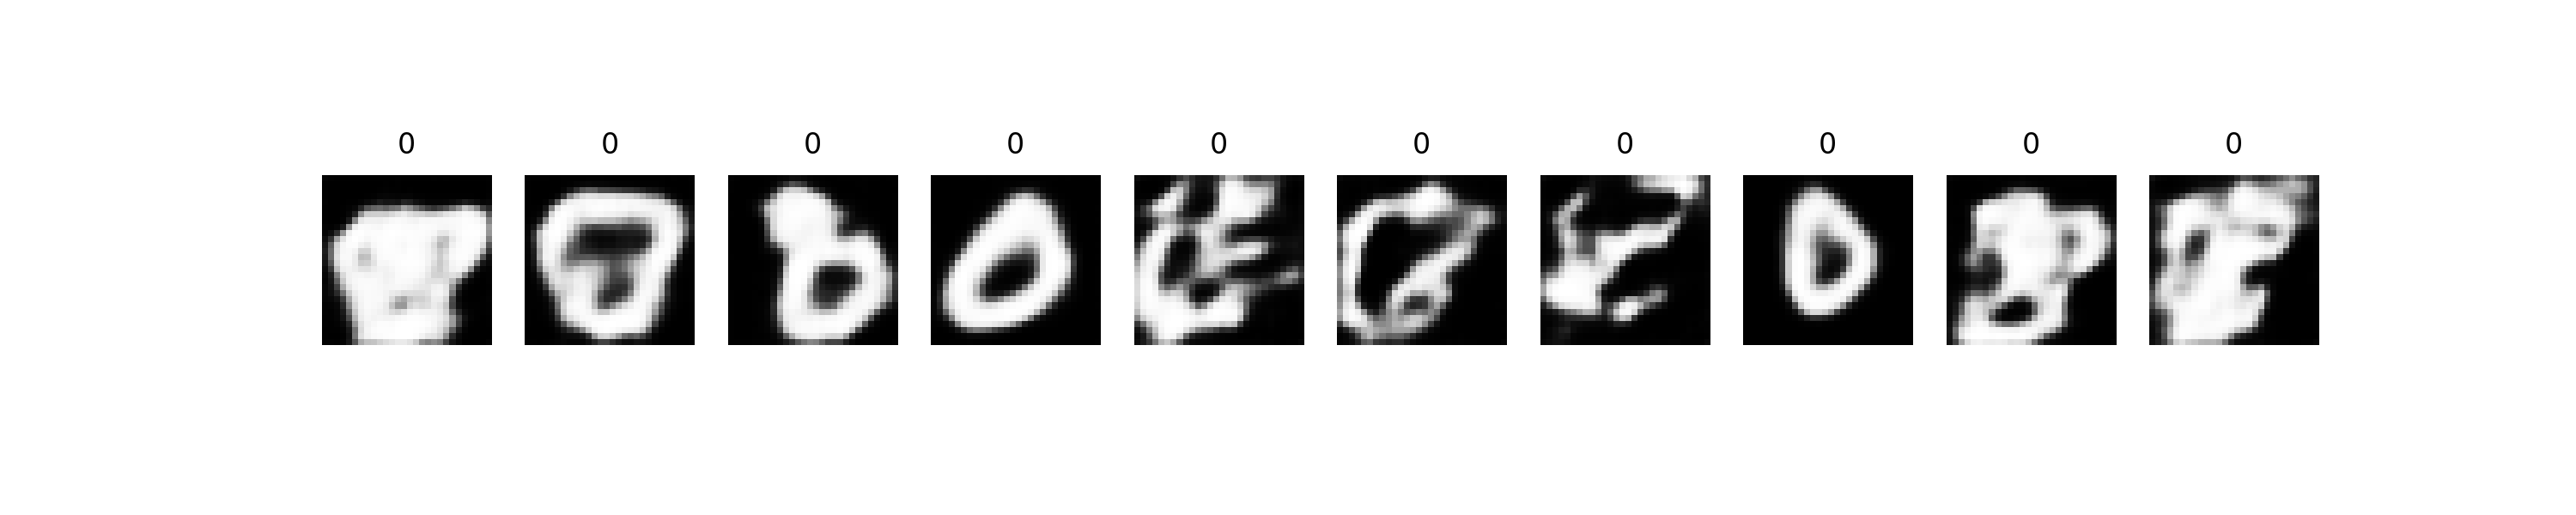
\includegraphics[width=\linewidth]{vae_run_2.png}
\caption{Generated samples from VAE Run 2.}
\label{fig:vae_run2}
\end{figure}

\begin{figure}[H]
\centering
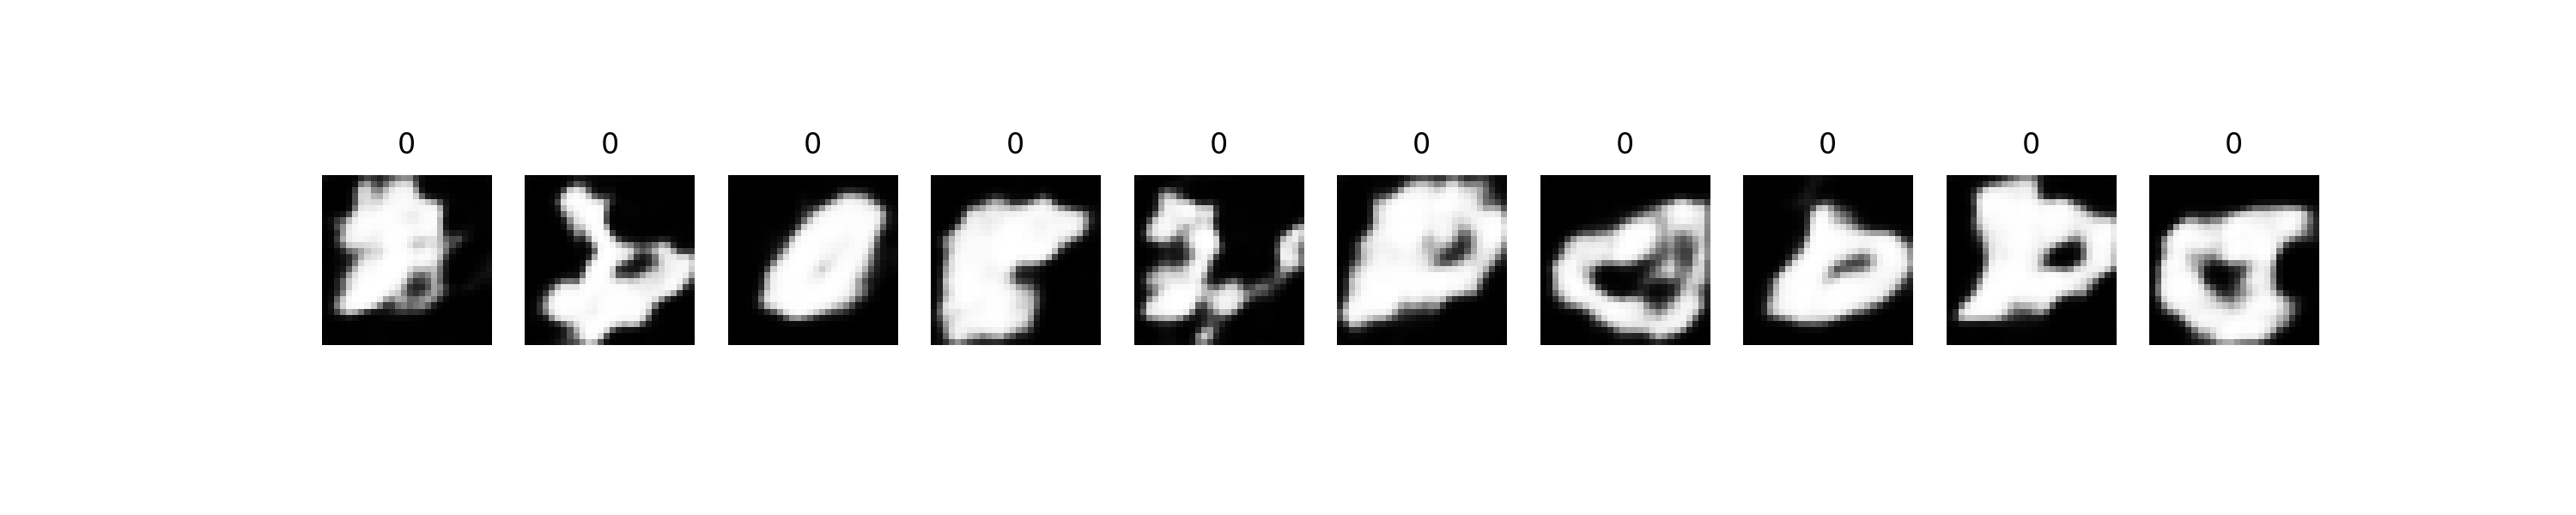
\includegraphics[width=\linewidth]{vae_run_3.png}
\caption{Generated samples from VAE Run 3.}
\label{fig:vae_run3}
\end{figure}

\begin{figure}[H]
\centering
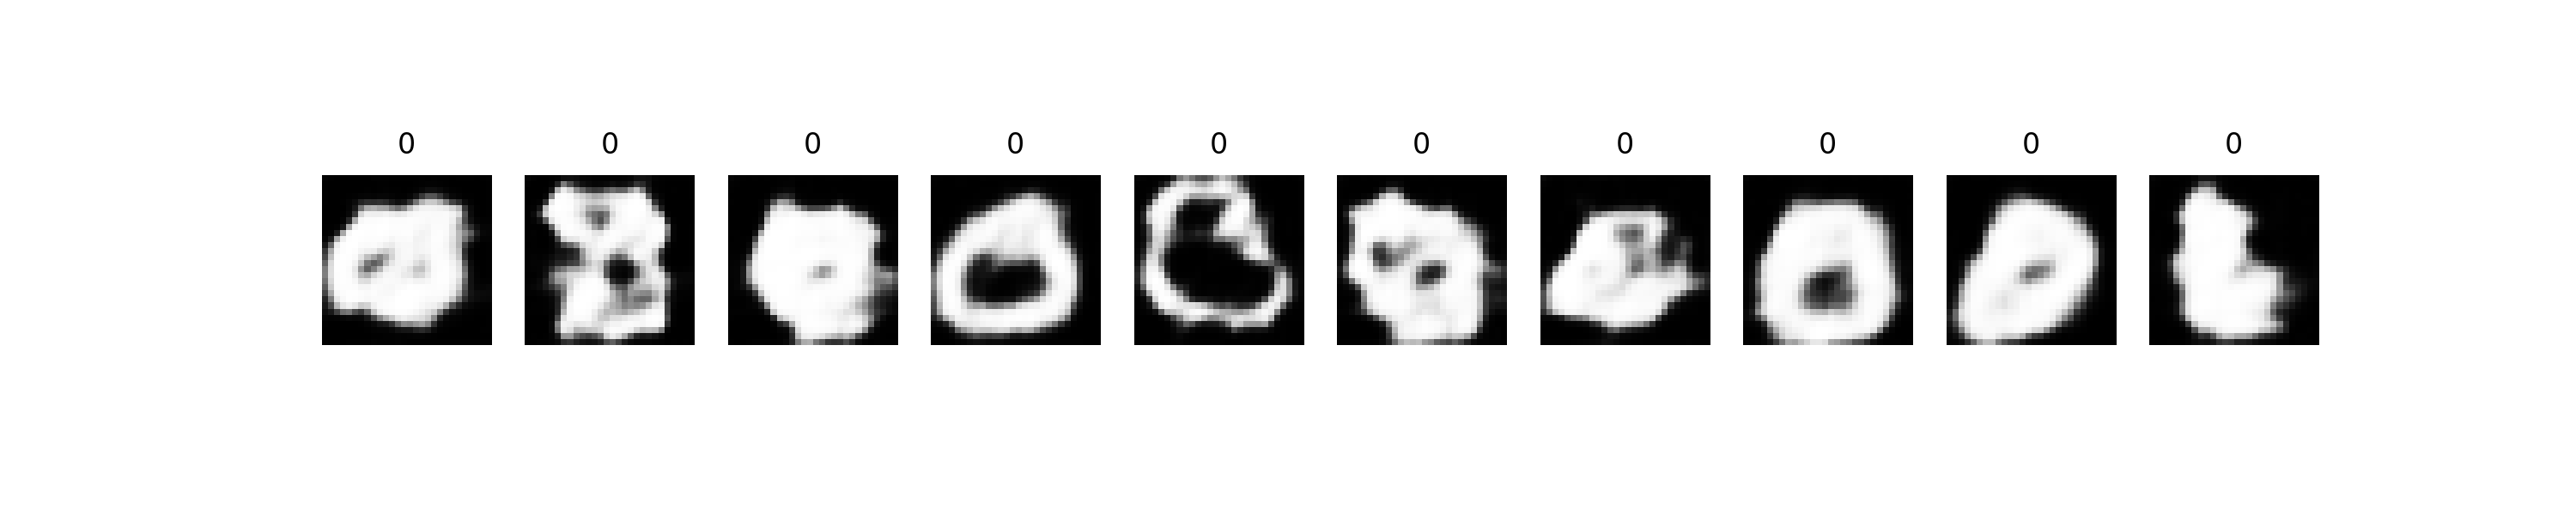
\includegraphics[width=\linewidth]{vae_run_4.png}
\caption{Generated samples from VAE Run 4.}
\label{fig:vae_run4}
\end{figure}

\begin{figure}[H]
\centering
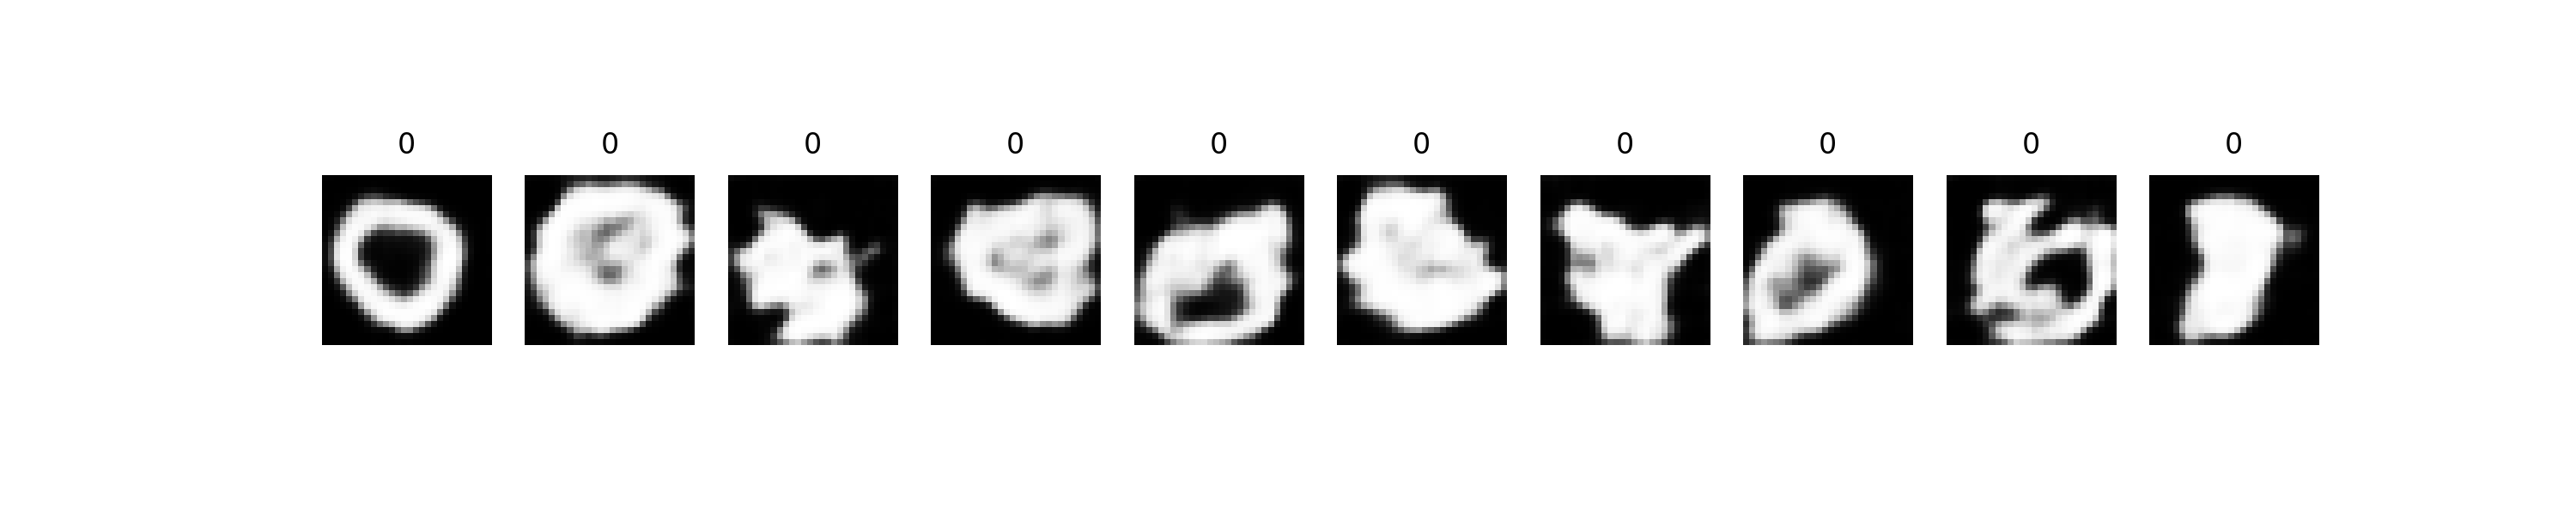
\includegraphics[width=\linewidth]{vae_run_5.png}
\caption{Generated samples from VAE Run 5.}
\label{fig:vae_run5}
\end{figure}

The generated images demonstrate that the Conditional VAE successfully learned the structural characteristics of handwritten digits while maintaining variation across samples.

% =====================================================
\subsubsection{Synthetic Dataset Construction}

Generated samples were filtered using the trained LeNet-5 classifier confidence.

Three datasets were created:

\begin{itemize}
    \item \textbf{Set A}: all generated samples
    \item \textbf{Set B}: high-confidence samples
    \item \textbf{Set C}: mid-confidence samples
\end{itemize}

% =====================================================
\subsubsection{Set A Samples}

\begin{figure}[H]
\centering
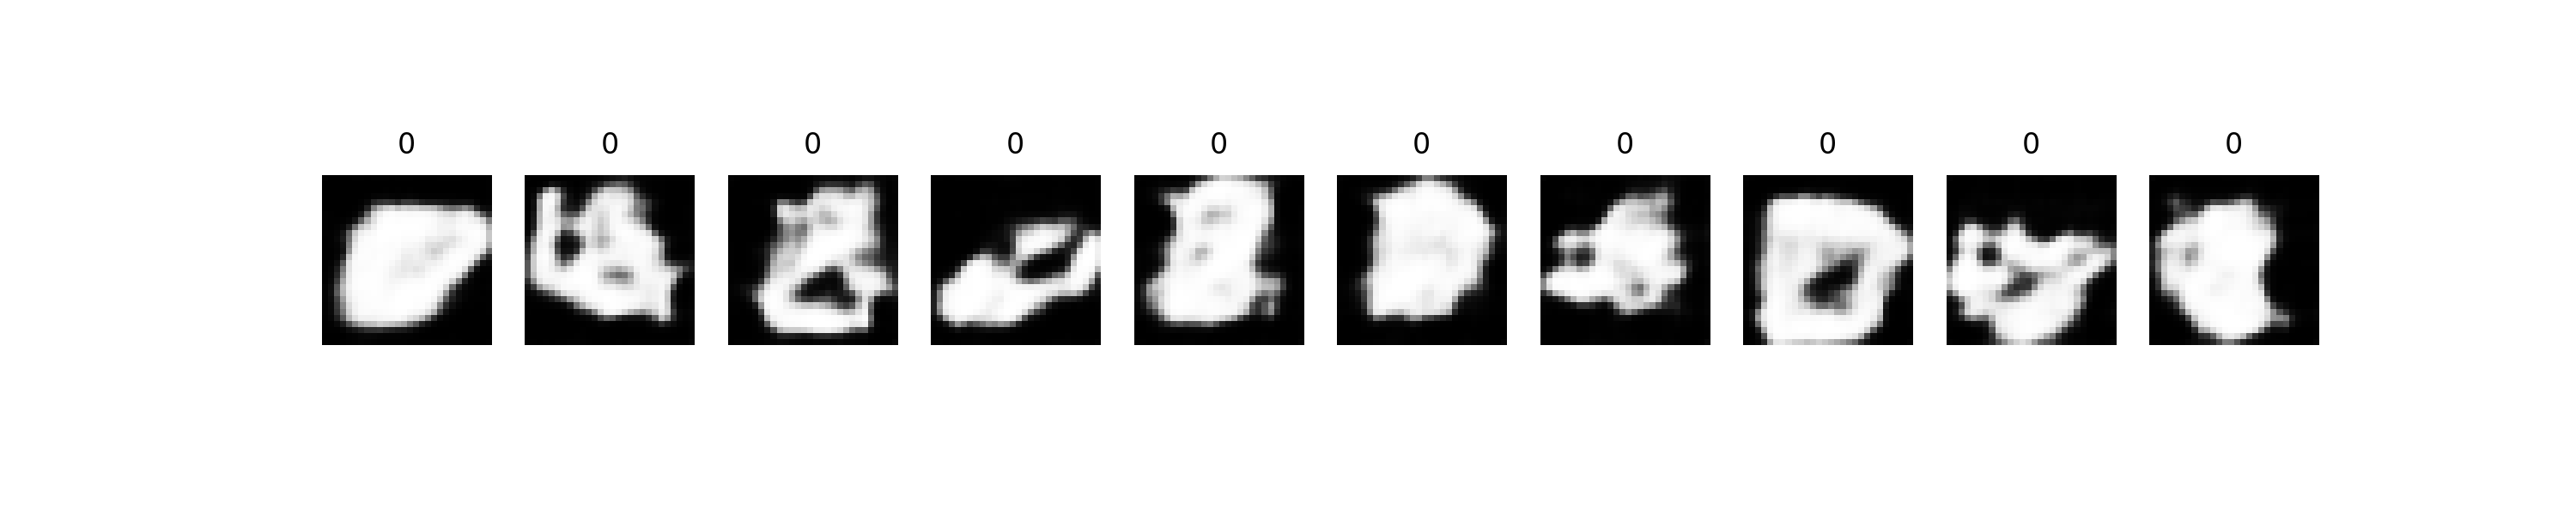
\includegraphics[width=\linewidth]{vae_setA.png}
\caption{Samples from Set A (all generated samples).}
\label{fig:setA}
\end{figure}

Set A contains all generated images without filtering. Some samples are realistic while others contain distortions and noisy structures.

% =====================================================
\subsubsection{Set B Samples}

\begin{figure}[H]
\centering
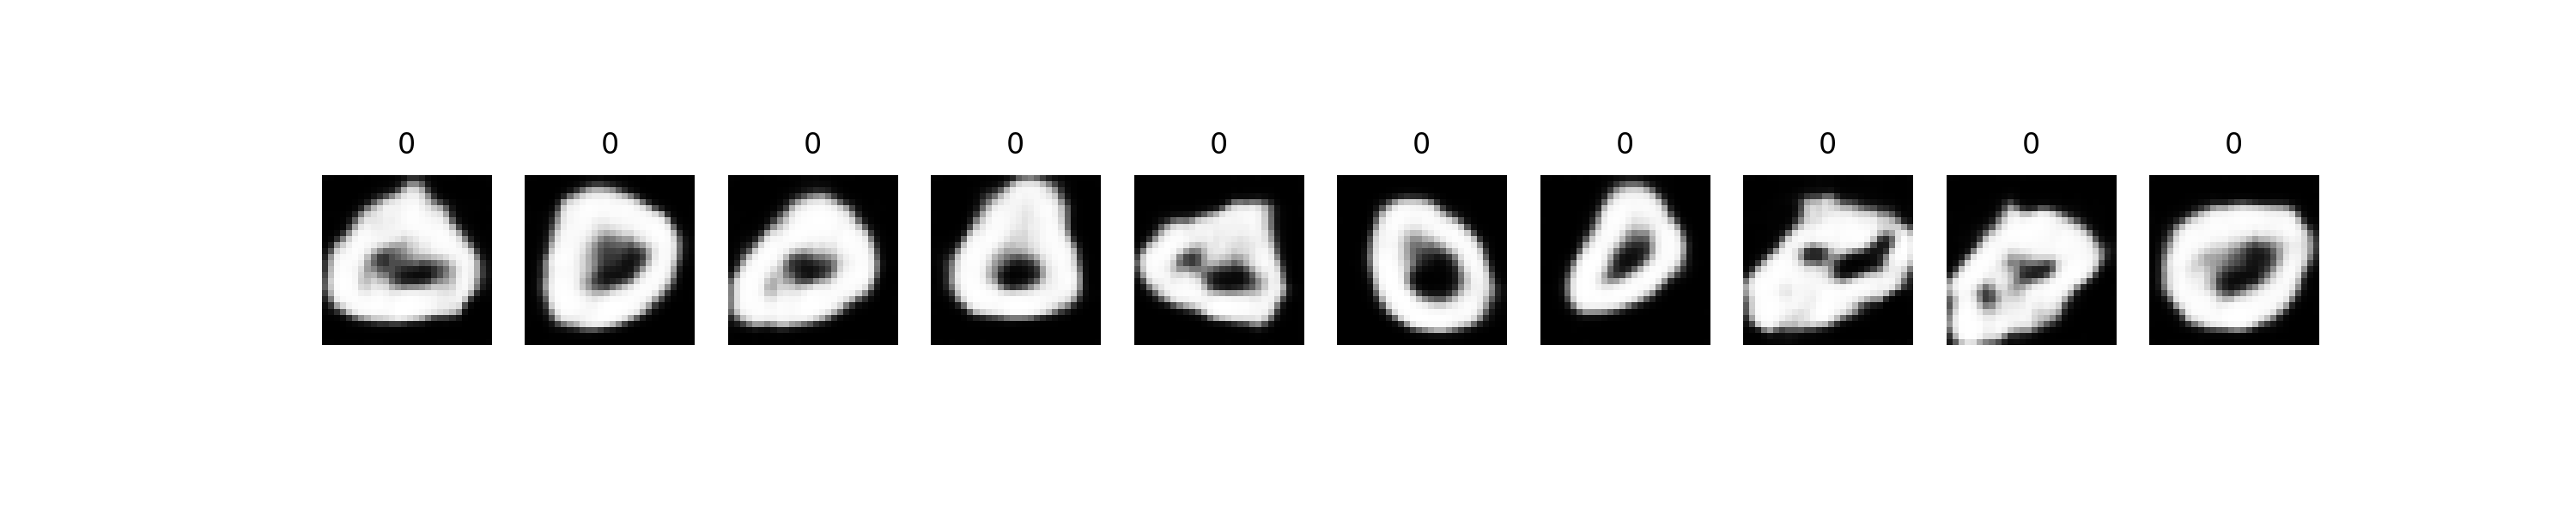
\includegraphics[width=\linewidth]{vae_setB.png}
\caption{Samples from Set B (high-confidence samples).}
\label{fig:setB}
\end{figure}

Set B contains cleaner and more realistic samples because only high-confidence predictions were accepted.

% =====================================================
\subsubsection{Set C Samples}

\begin{figure}[H]
\centering
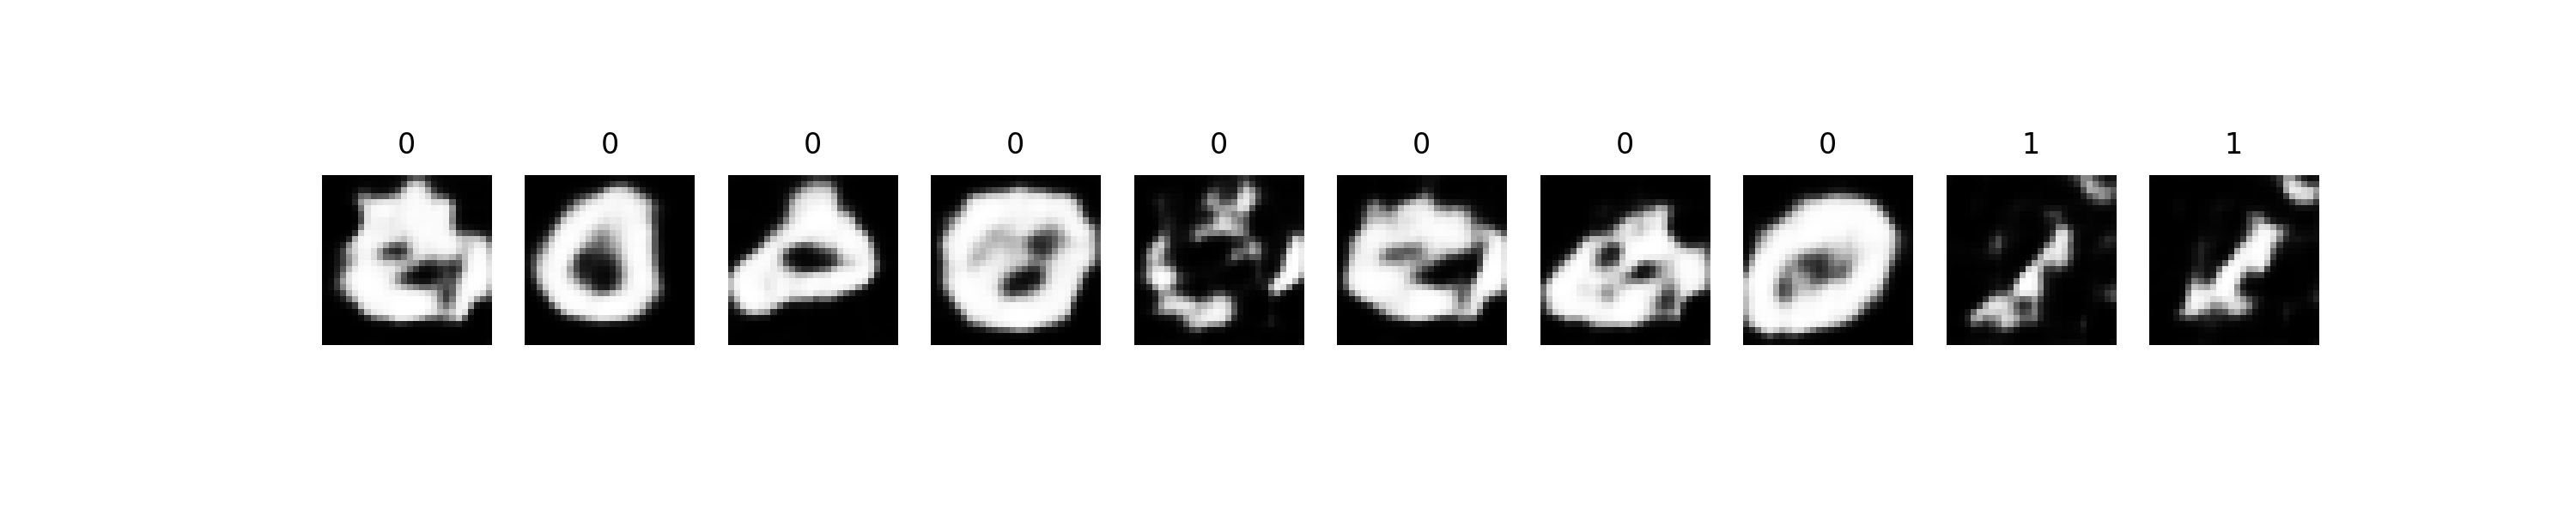
\includegraphics[width=\linewidth]{vae_setC.png}
\caption{Samples from Set C (mid-confidence samples).}
\label{fig:setC}
\end{figure}

Set C contains moderately confident samples that preserve diversity while removing highly corrupted outputs.

% =====================================================
\subsubsection{Experimental Results}

The final LeNet-5 classification accuracies are shown in Table~\ref{tab:vae_results}.

\begin{table}[H]
\centering
\caption{Comparison of classifier accuracy using different synthetic datasets.}
\label{tab:vae_results}

\begin{tabular}{|c|c|}
\hline
\textbf{Experiment} & \textbf{Accuracy} \\
\hline
350 Real Baseline & 96.36\% \\
\hline
Set A & 93.31\% \\
\hline
Set B & 95.25\% \\
\hline
Set C & 95.29\% \\
\hline
1000 Real Baseline & 98.17\% \\
\hline
\end{tabular}

\end{table}

% =====================================================
\subsubsection{Discussion}

The experimental results show that:

\begin{itemize}

\item Using only 350 real samples achieved a strong baseline accuracy of 96.36\%.

\item Adding all generated samples (Set A) reduced performance due to the inclusion of low-quality and distorted generated images.

\item Confidence filtering significantly improved performance.

\item Set B and Set C achieved accuracies close to the real-only baseline.

\item High-confidence filtering successfully removed unrealistic samples while preserving useful digit variations.

\item The 1000-real baseline still achieved the best performance because real samples preserve the true MNIST distribution more accurately than synthetic samples.

\end{itemize}

% =====================================================
\subsubsection{Conclusion}

A Conditional Variational Autoencoder was successfully implemented for MNIST handwritten digit generation.

The generated samples demonstrated that the VAE learned meaningful latent representations despite training on a very limited dataset.

Experimental evaluation showed that synthetic data quality strongly affects classifier performance. Confidence-based filtering improved the usefulness of generated samples and produced classification accuracy close to the real-only baseline.

The results indicate that VAE-generated data can partially compensate for limited datasets, although synthetic samples still do not fully replace real training data.

\endgroup